\chapter{Sprachdatenbanken}

\section{Stichworte zum Vortrag \em{Sprachdatenbanken}}

Archivierung, Annotation, Primär-, Sekundär- und Metadaten, Korpus, Repository, Validierung, Prävalidierung, Datensammlung, Datenaufbereitung

\section{Übungen}

\begin{figure}[htbp]
\begin{center}
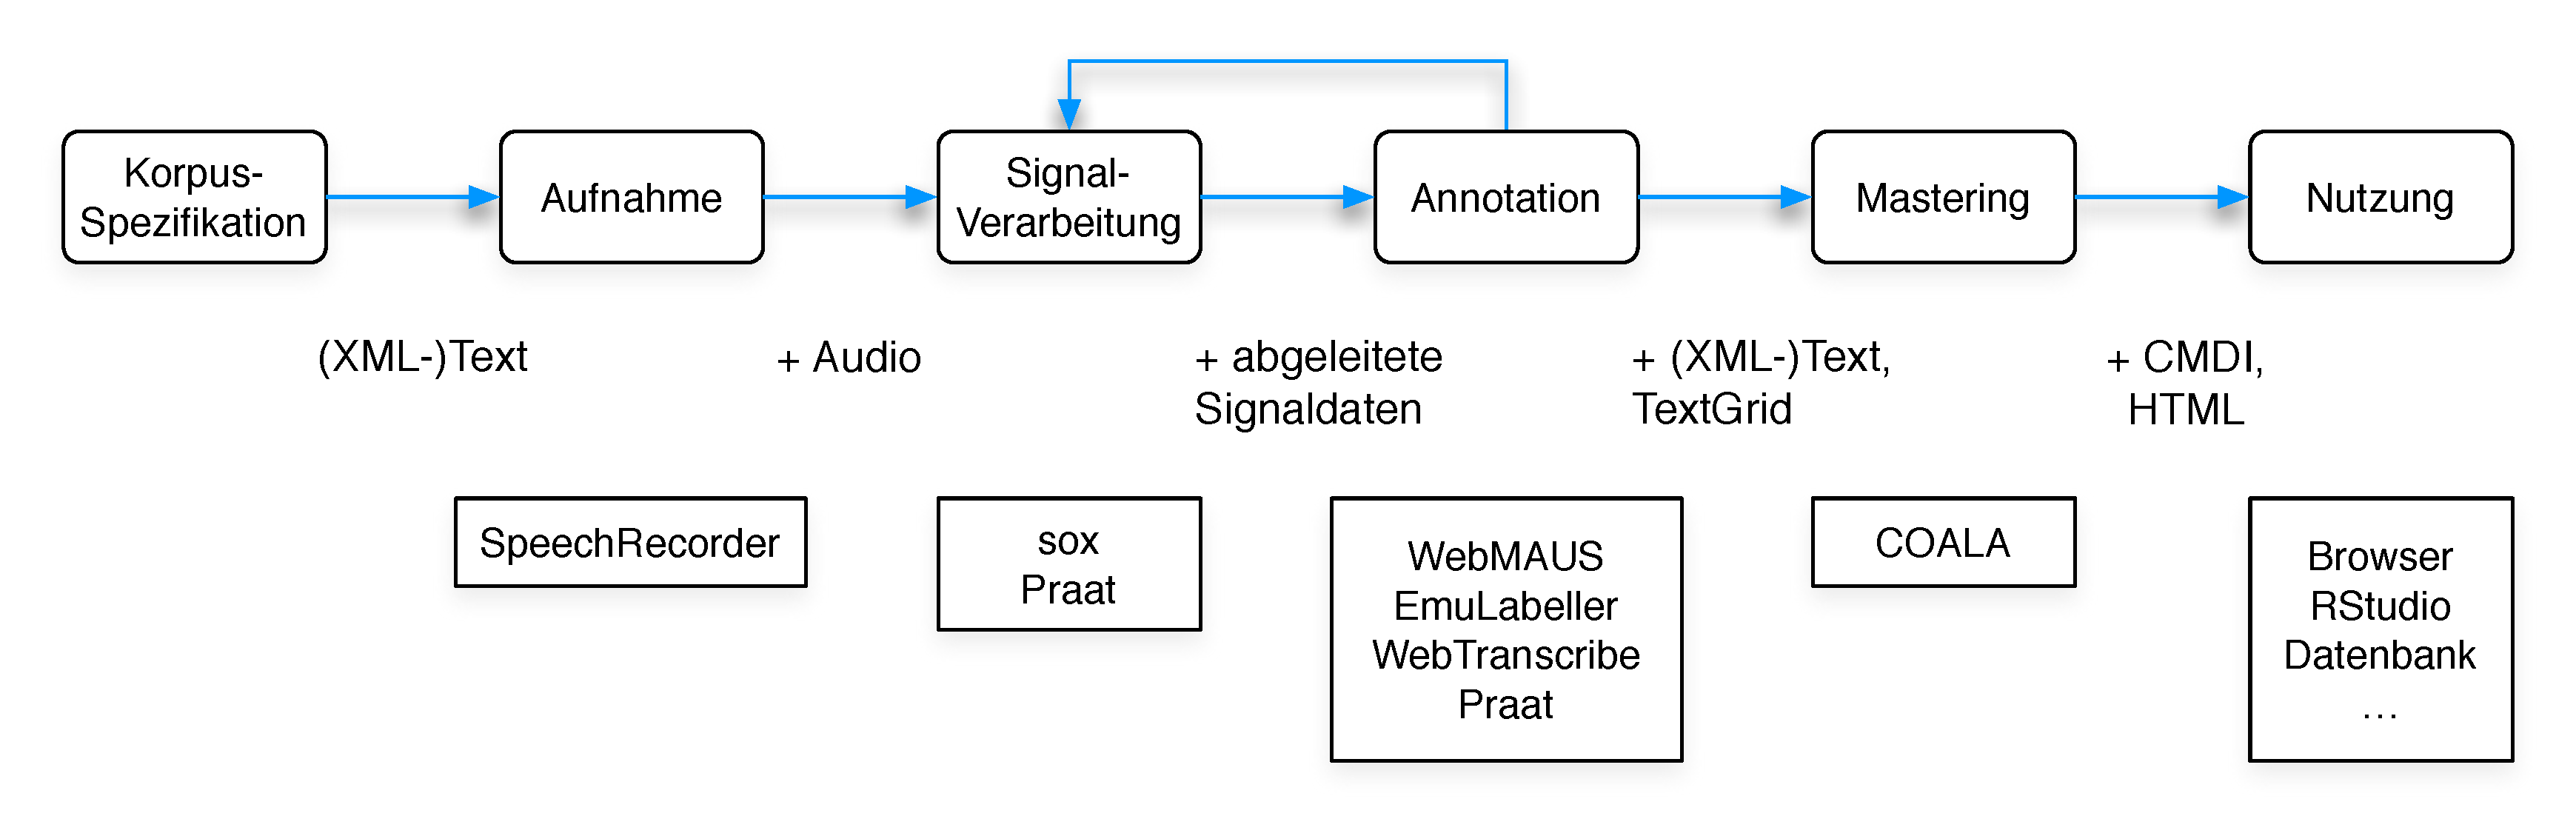
\includegraphics[width=1\textwidth]{grafiken/sprachdatenbanken/workflow-de-2.pdf}
\caption{Arbeitsablauf und Daten bei der Erstellung und Nutzung von Sprachdatenbanken. In den Kästchen stehen die Namen von Tools, die in diesem Arbeitsschritt häufig verwendet werden.}
\label{fig_sdb_arbeitsablauf}
\end{center}
\end{figure}

\newpage

\begin{enumerate}
\item{Welche Vorteile bieten web-basierte Sprachaufnahme und -annotation gegenüber traditionellen Verfahren?}
\vspace{5cm}
\item{Warum ist im Diagramm des Arbeitsablaufs (Abb. \ref{fig_sdb_arbeitsablauf}) ein Rückwärtspfeil von Annotation zu Signalverarbeitung?}
\vspace{5cm}
\item{Sind Sekundärdaten erweiterbar oder veränderbar? Wenn ja, wieso?}
\vspace{5cm}
\end{enumerate}

\newpage

\section{Literatur}

Bird, S.; Liberman, M. (2001). A Formal Framework for Linguistic Annotation. Speech Communication Band 33 Nr. 1,2. S.\,23-60. \newline\\
Bussmann, H. (1990). Lexikon der Sprachwissenschaft. Stuttgart: Körner Verlag.\newline\\
Draxler, C. (2008). Korpusbasierte Sprachverarbeitung. Tübingen: Narr Verlag. \newline\\
Schiel, F.; Draxler, C.; Baumann, A.; Ellbogen, T.; Steffen, A. (2003). The Production of Speech Corpora. Institut für Phonetik. LMU München.\newline\\
Schiel, F. (2003). The Validation of Speech Corpora. Institut für Phonetik. LMU München.


%\section{Links}
\label{link_clarin_repository}
{\tt clarin.phonetik.uni-muenchen.de/BASRepository/} (Stand: \today) Repository des Bayerischen Archivs für Sprachsignale am Institut für Phonetik der LMU.\newline\\
{\tt www.clarin.eu/content/virtual-language-observatory} (Stand: \today) Facettensuche nach Sprachdatenbanken.\newline\\
{\tt ldc.upenn.edu} (Stand: \today) Linguistic Data Consortium an der Universität von Pennsylvania.\newline\\
{\tt catalog.elra.info} (Stand: \today) Online Katalog der European Language Resources Asscociation.\newline\\
{\tt wals.info} (Stand: \today) World Atlas of Linguistic Structures online zur Dokumentation von Sprachstrukturen.
